\lecture{7}{17 March.}{}
\begin{remark}
    The requirement of \(f^{\prime} (x_0)\) is invertible is necessary to get the differentiability of \(f^{-1}\) at \(x_0\).  
\end{remark}

\section{The Implicit Function Theorem}
In \(\mathbb{R} ^2\), \(S = \left\{ (x, y) \mid x^2 + y^2 = 1 \right\} \) is a circle. However, \(S\) is not the graph of one function. \(S\) can be expressed as the union of the graph of four functions:
\[
    \begin{dcases}
        y = \sqrt{1 - x^2} \text{ for } -1 < x < 1 \\
        y = -\sqrt{1 - x^2} \text{ for } -1 < x < 1 \\
        x = \sqrt{1 - y^2} \text{ for } -1 < y < 1 \\
        x = - \sqrt{1 - y^2} \text{ for }  -1 < y < 1.       
    \end{dcases}
\]    
For a \(\mathbb{R} ^3\) case, consider \(S = \left\{ (x, y, z) \mid x^2 + y^2 - z^2 + 1 = 0 \right\} \), then \(S\) is the union of \(2\) graph:
\[
    \begin{dcases}
        z = \sqrt{x^2 + y^2 + 1} \text{ for } z > 0 \\
        z = -\sqrt{x^2 + y^2 + 1} \text{ for } z < 0.   
    \end{dcases}
\]   

\begin{center}
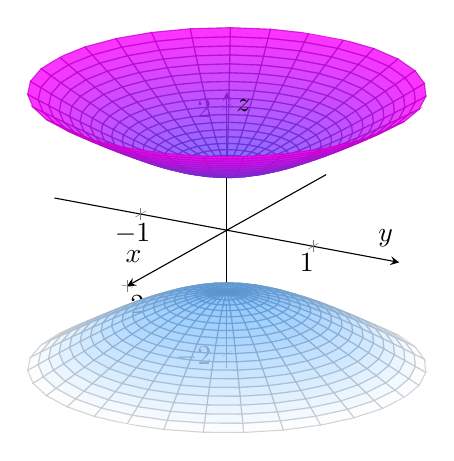
\begin{tikzpicture}
\begin{axis}[
  width=0.7\linewidth,
  view={120}{25},
  axis lines=center,
  xlabel={$x$},
  ylabel={$y$},
  zlabel={$z$},
  domain=0:360,
  y domain=0:2,
  samples=32,
  samples y=20,
  colormap/cool,
  z buffer=sort,
  grid=major
]
  \addplot3[
    surf,
    opacity=0.8
  ]
  ({y*cos(x)},{y*sin(x)},{sqrt(y^2+1)});

  \addplot3[
    surf,
    opacity=0.8
  ]
  ({y*cos(x)},{y*sin(x)},{-sqrt(y^2+1)});
\end{axis}
\end{tikzpicture}
\end{center}

For another example, consider \(S = \left\{ (x, y, z) \mid x^2 + y^2 = \cosh^2(z) \right\} \), where 
\[
    \cosh(z) = \frac{e^z + e^{-z}}{2}.
\]
Then \(S\) is symmetric with respect to \(z\). 

\begin{center}
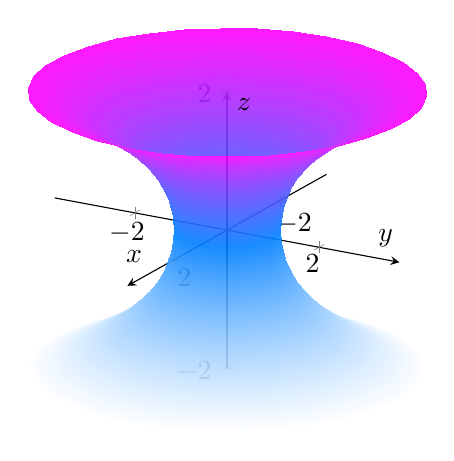
\begin{tikzpicture}
\begin{axis}[
  width=0.7\linewidth,
  view={120}{25},
  axis lines=center,
  xlabel={$x$},
  ylabel={$y$},
  zlabel={$z$},
  domain=0:360,
  y domain=-2:2,
  samples=35,
  samples y=25,
  colormap/cool,
  z buffer=sort,
  grid=major
]
  \addplot3[
    surf,
    opacity=0.9,
    shader=interp
  ]
  ({cosh(y)*cos(x)},{cosh(y)*sin(x)},{y});
  
\end{axis}

\end{tikzpicture}
\end{center}

\begin{theorem}[Implicit Function Theorem]
    Let \(E\) be an open subset of \(\mathbb{R} ^n\), let \(f:E \to \mathbb{R} \) be continuously differentiable, and let \(y = (y_1, y_2, \dots , y_n) \in E\) s.t. \(f(y) = 0\) and \(\frac{\partial f(y)}{\partial x_n} \neq 0\). Then, \(\exists \) an open subset \(U \subseteq \mathbb{R} ^{n-1}\) containing \((y_1, y_2, \dots , y_{n-1})\), an open subset \(V \subseteq E\) containing \(y\), and a function \(g: U \to \mathbb{R} \) s.t.
    \[
        g(y_1, y_2, \dots , y_{n-1}) = y_n
    \]          
    and 
    \[
        \left\{ x = (x_1, \dots , x_n) \in V: f(x) = 0 \right\} = \left\{ (x_1, \dots , x_{n-1}, g(x_1, \dots , x_{n-1})) : (x_1, \dots ,x_{n-1}) \in U \right\}.  
    \]
    In other words, the set \(\left\{ x \in V: f(x) = 0 \right\} \) is a graph of a function over \(U\). Moreover, \(g\) is differentiable at \((y_1, \dots , y_{n-1})\) and we have 
    \[
        \frac{\partial g}{\partial x_{j} } (y_1, y_2, \dots , y_{n-1}) = -\frac{\frac{\partial f}{\partial x_j}(y) }{\frac{\partial f}{\partial x_n}(y) } 
    \]    
    for all \(1 \le j \le n - 1\). 
\end{theorem}

\begin{proof}
    Define \(F: E \to \mathbb{R} ^n\) by 
    \[
        (x_1, x_2, \dots , x_n) \to (x_1, x_2, \dots , x_{n-1}, f(x_1, x_2, \dots , x_{n})).
    \] 
    Since \(f \in C^1(E)\), so \(F \in C^1(E)\). Thus,
    \[
        DF(x) = \begin{bmatrix}
             \nabla x_1 \\
             \nabla x_2 \\
             \vdots \\
             \nabla x_{n-1} \\
             \nabla f
        \end{bmatrix} = \begin{bmatrix}
            1 & 0 & \cdots & 0  \\
            0 & 1 & \cdots & 0  \\
             &  & \ddots &   \\
            0 & \cdots & 1 & 0  \\
            \frac{\partial f}{\partial x_1}(x)  & \dots  & \frac{\partial f}{\partial x_{n-1}}(x)  & \frac{\partial f}{\partial x_n}(x)   \\
        \end{bmatrix},
    \]  
    which gives 
    \[
        \det (DF(x)) = \frac{\partial f(x)}{\partial x_n}. 
    \]
    Hence, 
    \[
        \det (DF(y)) = \frac{\partial f (y)}{\partial x_n} \neq 0,
    \]
    so \(F^{\prime} (y)\) is invertible. Now we can apply inverse function theorem, so \(\exists \) an open set \(V \subseteq E\) and \(W \subseteq \mathbb{R} ^m\) with \(y \in V\) and \(F(y) = (y_1, \dots , y_{n-1}, 0) \in W\) s.t. \(F: V \to W\) is a \(C^1\) diffeomorphism. Write the inverse in coordinate
    \[
        F^{-1}( \underbrace{u_1, u_2, \dots , u_n}_{u} )  = (h_1(u), h_2(u), \dots , h_n(u)).
    \] 
    Since \(F(F^{-1}(u)) = u\) for \(u \in W\), so 
    \[
        (h_1(u), \dots h_{n-1}(u), f(h_1(u), \dots , h_n(u))) = F(h_1(u), h_2(u), \dots , h_n(u)) = (u_1, u_2, \dots, u_n).
    \]
    Hence,
    \begin{align*}
        h_1(u) &= u_1 \\
        h_2(u) &= u_2 \\
        &\vdots \\
        h_{n-1}(u) &= u_{n-1}\\
        f(h_1(u), \dots , h_n(u)) &= f(u_1, u_2, \dots , u_{n-1}, h_n(u)) = u_n.
    \end{align*} 
    Thus, for \(u_1, \dots , u_n \in W\), 
    \[
        F^{-1}(u_1, \dots , u_n) = (u_1, \dots , u_{n-1}, h_n(u)).
    \]         
    By this, we can plug \(u_n = 0\) into it and get 
    \[
        F^{-1}(u_1, \dots , u_{n-1}, 0) = (u_1, \dots , u_{n-1}, h_n(u_1, \dots , u_{n-1}, 0)),
    \] 
    where 
    \[
        0 = u_n = f(u_1, \dots , u_{n-1}, h_n(u_1, \dots , u_{n-1}, 0)).
    \]
    Now we want to restrict \(u_n = 0\) and define \(g\). Set 
    \[
        U = \left\{ x^{\prime} = (x_1, \dots , x_{n-1}) \in \mathbb{R} ^{n-1}, (x^{\prime} , 0) \in W \right\}.
    \]  
    Then \(U\) is open and contains \((y_1, \dots , y_{n-1})\) since 
    \[
        F(y_1, \dots , y_n) = (y_1, \dots , y_{n-1}, f(y_1, \dots , y_n)) = (y_1, \dots , y_{n-1}, 0) \in W.
    \]
    Define \(g: U \to \mathbb{R} \) by 
    \[
        g(x^{\prime} ) = g(x_1, \dots , x_{n-1}) = h_n(x_1, \dots , x_{n-1}, 0).
    \]   
    Since \(f(y_1, \dots , y_n) = 0\), we know \(F(y) = (y_1, \dots , y_n, 0)\). Hence,
    \begin{align*}
        (y_1, \dots , y_n) &= y = F^{-1}(F(y)) = F^{-1}(y_1, \dots , y_n, 0) = (y_1, \dots , y_{n-1}, h_n(y_1, \dots , y_{n-1}, 0 ) ).
    \end{align*}  
    Thus,
    \[
        y_n = h_n(y_1, \dots , y_{n-1}, 0) = g(\underbrace{y_1, \dots , y_{n-1}}_{y^{\prime} }) \implies g(y^{\prime} ) = y_n.
    \]
    Moreover, \(g\) is differentiable since \(h_n\) is differentiable. 

    Now we want to show the zero set is the graph of \(g\). 

    \begin{claim}
        \(\left\{ x \in V: f(x) = 0 \right\} = \left\{ (x^{\prime} , g(x^{\prime} )): x^{\prime} \in U \right\}  \). 
    \end{claim}   
    \begin{explanation}
        Let \(A = \left\{ x \in V: f(x) = 0 \right\}\) and \(B = \left\{ (x^{\prime} , g(x^{\prime} )): x^{\prime} \in U \right\}\). We first show \(A \subseteq B\). Let \(x = (x^{\prime} , x_n) \in V\) and \(f(x^{\prime} , x_n) = 0\). Then 
        \[
            F(x) = (x^{\prime} , f(x^{\prime} , x_n)) = (x^{\prime} , 0) \in W.
        \]     
        Since \(x^{\prime} \in U\),
        \[
            x = F^{-1}(F(x)) = F^{-1} (x^{\prime} , 0) = (x^{\prime} , h_n(x^{\prime} , 0)) = (x^{\prime} , g(x^{\prime})).
        \]
        Hence, \(A \subseteq B\).  

        Now we show \(B \subseteq A\). Suppose \(x^{\prime} \in U\), then 
        \[
            x = (x^{\prime} , g(x^{\prime} )) = (x^{\prime} , h_n(x^{\prime} , 0)).
        \]  
        Thus,
        \[
            F^{-1}(x^{\prime} , 0) = (x^{\prime} , h_n(x^{\prime} , 0)) = (x^{\prime} , g(x^{\prime} )).
        \]
        Thus,
        \[
            (x^{\prime} , 0) = F(F^{-1}(x^{\prime} , 0)) = F(x^{\prime} , g(x^{\prime} )) = (x^{\prime} , f(x^{\prime} , g(x^{\prime} ))).
        \]
        Thus,
        \[
            f(x^{\prime} , g(x^{\prime} )) = 0,
        \]
        which shows \(x \in A\). 
    \end{explanation}

    Now for \((x_1, x_2, \dots , x_{n-1}) \in U\), we know
    \[
        f(x_1, x_2, \dots , x_{n-1}, g(x_1, x_2, \dots , x_{n-1})) = 0.
    \] 
    Fix \(j \in [n - 1]\), and set \(y^{\prime} = (y_1, \dots , y_{n-1})\). Consider 
    \[
        \psi (t) \coloneqq f(y^{\prime} + te_j, g(y^{\prime} + te_j)),
    \]  
    defined for \(t\) near \(0\). Note that \(\psi (t) \equiv 0\) for all \(t\) sufficiently close to \(0\). Hence, \(\psi ^{\prime} (0) = 0\). Since \(f\) is differentiable at \(y = (y^{\prime} , g(y^{\prime} ))\) and \(g\) is differentiable at \(y^{\prime} \), we may apply the chain rule to compute \(\psi ^{\prime} (0)\). Suppose \(\psi (t) = f(\gamma (t))\), where \(\gamma : \mathbb{R} \to \mathbb{R} ^n\) is defined by 
    \[
        t \mapsto (y^{\prime} + te_j, g(y^{\prime} + te_j)).
    \]   
    Now since
    \[
        \psi ^{\prime} (t) = f^{\prime} (\gamma (t)) \circ \gamma ^{\prime} (t),
    \]
    and \(f\) is a function from a subset of \(\mathbb{R} ^n\) to \(\mathbb{R} \), so
    \[
        f^{\prime} (\gamma (t)) = \nabla f(\gamma (t)) = \left( \frac{\partial f(\gamma (t))}{\partial x_1}, \frac{\partial f(\gamma (t))}{\partial x_2}, \dots , \frac{\partial f(\gamma (t))}{\partial x_n}  \right), 
    \]    
    which gives
    \[
        f^{\prime} (\gamma (0)) = \left( \frac{\partial f(y)}{\partial x_1}, \frac{\partial f(y)}{\partial x_2}, \dots , \frac{\partial f(y)}{\partial x_n}  \right). 
    \]
    Also, 
    \[
        \gamma ^{\prime} (t) = \left( 0, \dots , 1, \dots , 0, \frac{\mathrm{d} g(y^{\prime}  + te_j)}{\mathrm{d}t} \right) \implies \gamma ^{\prime} (0) = \left( 0, \dots , 1, \dots , 0, \frac{\mathrm{d} g(y^{\prime})}{\mathrm{d}t} \right), 
    \]
    and note that 
    \[
       \frac{\mathrm{d} g(y^{\prime}  + te_j)}{\mathrm{d}t} = \nabla g(y^{\prime} + te_j) \circ e_j \implies \frac{\mathrm{d} g(y^{\prime} )}{\mathrm{d}t} = \nabla g(y^{\prime} ) \circ e_j = \frac{\partial g(y^{\prime} )}{\partial x_j}.   
    \]
    Hence, 
    \begin{align*}
        \psi ^{\prime} (0) &=  \left( \frac{\partial f(y)}{\partial x_1}, \frac{\partial f(y)}{\partial x_2}, \dots , \frac{\partial f(y)}{\partial x_n}  \right) \circ \left( 0, \dots , 1, \dots , 0, \frac{\partial g(y^{\prime} )}{\partial t}  \right) \\
        &= \frac{\partial f}{\partial x_j}(y) + \frac{\partial f}{\partial x_n}(y) \frac{\partial g}{\partial x_j}(y^{\prime} ),
    \end{align*}        
    and thus 
    \[
       0 = \psi ^{\prime} (0) = \frac{\partial f}{\partial x_j}(y) + \frac{\partial f}{\partial x_n}(y) \frac{\partial g}{\partial x_j}(y^{\prime} ). 
    \]
    Now since \(\frac{\partial f}{\partial x_n}(y) \neq 0 \), we have 
    \[
        \frac{\partial g}{\partial x_j}(y^{\prime} ) = -\frac{\frac{\partial f}{\partial x_j}(y) }{\frac{\partial f}{\partial x_n}(y) }. 
    \]  
\end{proof}

\begin{eg}
    Let \(S = \left\{ (x, y, z) \in \mathbb{R} ^3 \mid xy + yz + xz = -1 \right\} \), which we rewrite as 
    \[
        \left\{ (x, y, z) \in \mathbb{R} ^3 : f(x, y, z) = 0 \right\} ,
    \]
     where \(f: \mathbb{R} ^3 \to \mathbb{R} \) is the function 
    \[
        f(x, y, z) = xy + yz + xz + 1.
    \]      
    Clearly \(f\) is continuously differentiable, and \(\frac{\partial f}{\partial z} = y + x \). Thus, for any \((x_0, y_0, z_0) \in S\) sith \(y_0 + x_0 \neq 0\), one can write this surface (near \((x_0, y_0, z_0)\)) as a graph of the form 
    \[
        \left\{ (x, y, g(x, y)) : (x, y) \in U \right\} 
    \]   
    for some open set \(U\) containing \((x_0, y_0)\), and some function \(g\) which is differentiable at \((x_0, y_0)\). Indeed one can implicitly obtain
    \[
        \frac{\partial g}{\partial x} (x_0, y_0) = - \frac{y_0 + z_0}{y_0 + x_0}, \quad \text{and} \quad \frac{\partial g}{\partial y}(x_0, y_0) = -\frac{x_0 + z_0}{y_0 + x_0}.    
    \]    
\end{eg}